Theoretical immigration effects. 

\begin{enumerate}[label=(\alph*)]

\item 
Suppose that immigrant programmers have labor supply functions identical to natives’ supply functions and that employers treat immigrant and native programmers as perfect substitutes. Use graphs to show the effect of an influx of $n_2$ immigrants on native programmers.

First let's suppose a linear function for the labor supply $h(w) = w$ . Therefore $S_1 = n_1h(w) = n_1w ; S_2 = n_2h(w)=n_2w$. If we add up both labor supply functions which correspond to the natives and immigrants respectively we will have $S = (n_1 + n_2)w \ \text{or} \ w =\frac{1}{n_1 + n_2}S $ so the labor supply function will experience a change on the slope, which is different than an increase of immigrants who supply labor inelastically . The latter means just a right parallel shift .  

\begin{figure}[H]
    \centering
    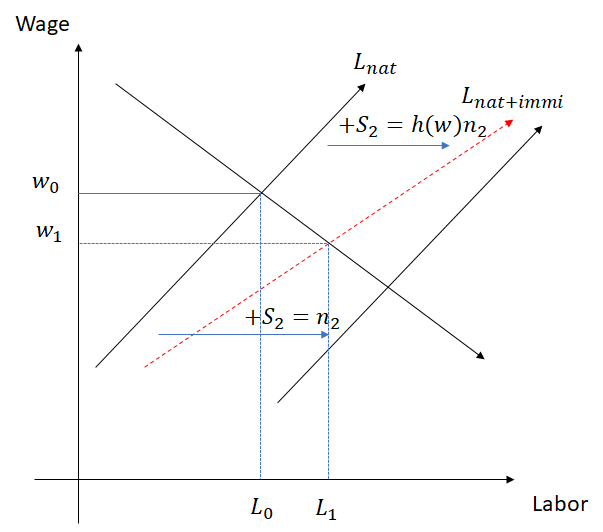
\includegraphics[width=0.55\textwidth]{Images/immigrant_effect.png}
    \caption{Effect of Immigrant supply}
    \label{fig:immigrants}
\end{figure}


\item 
By totally differentiating equilibrium conditions, derive comparative statics formulas for the elasticity of native wages and employment with respect to immigration Which economic parameters govern immigration effects? Since both type of workers have the same labor supply functions,and taking total differentiation 

\begin{equation}
\begin{aligned}
 & D(w) = n_1h(w) + n_2h(w) ;\ \text{where}  \ S_1 = n_1h(w) , S_2 = n_2h(w)  \\
 & D'(w)dw = n_1h'(w)dw + h(w)dn_1 +n_2h'(w)dw + h(w)dn_2
\end{aligned}
\end{equation}

Divide by $D(w)$ ,multiply by $\frac{w}{w}$, $\frac{n_2}{n_2}$

\begin{equation}
\begin{aligned}
 & \frac{D'(w)wdw}{D(w)w}  =  \frac{n_1h'(w)w}{S_1(w)}\frac{S_1(w)}{D(w)}\frac{dw}{w} +
 \frac{n_2h'(w)w}{S_2(w)}\frac{S_2(w)}{D(w)}\frac{dw}{w} +
 \frac{n_2h(w)}{D(w)}\frac{dn_2}{n_2} \\
 & \eta dln(w) = \epsilon_1(1-\phi)dln(w) + \epsilon_2\phi dln(w) + \phi dln(n_2)
\end{aligned}
\end{equation}


therefore the effects of immigration on wages is :

\begin{equation}
\begin{aligned}
\frac{dln(w)}{dln(n_2)} = \frac{\phi}{\eta - \epsilon_1 + \phi(\epsilon_1 - \epsilon_2)}
\end{aligned}
\end{equation}

when both types of workers have the same labor supply $\epsilon_1 = \epsilon_2$, the effects on wages will be govern positively by the immigrant share $\phi$ and the elasticity supply $\epsilon_1$ but will have a negative relation with the elasticity demand $\eta$.
It would be useful to see the effects on the employment 

\begin{equation}
\begin{aligned}
\frac{dL_1}{dn_2} = \frac{dln(S_1)}{dln(S_1)}\frac{S_1}{S_2} =   \frac{\epsilon(1-\phi) }{\eta - \epsilon_1 + \phi(\epsilon_1 - \epsilon_2)}
\end{aligned}
\end{equation}


\end{enumerate}